\section*{如何阅读本文档}
下面给出了本文档的结构,单击目录树上的节点便可以查看文档的相关部分。
%\dirtree{%
%.1 intro.
%.2 a. 
%.1 b. 
%.2 c. 
%.3 d. 
%}
\label{pagetree}
\DTsetlength{1em}{5em}{0.3em}{1pt}{1.6pt}
\renewcommand*\DTstyle{\ttfamily}
\dirtree{%
.1 \hyperref[pagetree]{Unicore-MiniC 编译器}.
.2 \hyperref[flexbison]{词法、语法分析}.
.3 \hyperref[flex]{词法分析, flex}.
.3 \hyperref[bison]{语法分析, bison}.
.3 \hyperref[syntexerror]{语法错误检查}.
.3 \hyperref[pitfallc1]{谬误与陷阱}.
.2 \hyperref[intermidiate]{中间表示}.
.3 \hyperref[AST]{抽象语法树AST}.
.4 \hyperref[genAST]{生成}.
.4 \hyperref[symtbl]{符号表}.
.5 \hyperref[declchk]{声明错误检查}.
.4 \hyperref[typeveri]{类型检查}.
.3 \hyperref[triple]{三元式表示}.
.4 \hyperref[tripleinst]{三元式指令列表}.
.4 \hyperref[triplestruct]{三元式结构}.
.4 \hyperref[ASTtotriple]{将AST转化为三元式}.
.4 \hyperref[basicblock]{生成基本块}.
.3 \hyperref[indepopt]{机器无关优化}.
.4 \hyperref[peephole:intermidiate]{窥孔优化}.
.4 \hyperref[dataflow]{数据流分析}.
.3 \hyperref[pitfallc2]{谬误与陷阱}.
.2 \hyperref[targetcode]{目标代码}.
.3 \hyperref[targetmachine]{编译器-目标机器接口与二进制规范}.
.3 \hyperref[registeralloc]{寄存器分配}.
.3 \hyperref[tripletotarget]{三元式转换为目标代码}.
.3 \hyperref[depopt]{机器相关优化}.
.4 \hyperref[peephole:target]{窥孔优化}.
.4 \hyperref[tailrecursion]{尾递归优化}.
.4 \hyperref[assembledispatch]{指令调度}.
.3 \hyperref[tarpitc3]{谬误与陷阱}.
.2 \hyperref[joint]{编译-体系联合实验}.
%.3 系统调用.
}
\section*{本文档包括的内容}
本文档的目标\emph{并不是}用于展示MiniC冗杂的代码,而是提供一个概括的全局视角来了解这个实习项目。\\
文档涵盖了如下的几个方面:
\begin{itemize}
	\item Unicore-MiniC编译器(以下在没有歧义的情况下简称之为MiniC)的总体设计方案
	\item MiniC的各个单元的设计方案,包括主要的数据结构和重要的算法
	\item MiniC各个单元之间的协同关系
	\item 为相关代码的阅读提供的指引
	\item 在开发过程中遇到的困难,遭遇的陷阱和付出的代价\footnote{参见某些章中的“谬误与陷阱”一节}
\end{itemize}
\section*{\textsc{MiniC In a Nutshell}}
\subsection*{项目目标}
\begin{itemize}
	\item 输入MiniC源代码,输出Unicore32汇编代码
	\item 利用Unicore32二进制工具链中的链结器链接后的程序能在 Unicore32 实体机器上运行
	\item 链接后的程序能够在同时设计的 Unicore32 模拟器上运行
	\item 通过对模拟器相关参数、指令系统的修改,考察编译-ISA 对性能的综合影响
\end{itemize}
整个项目将全部以C语言实现,用\verb|gcc|进行编译;以\verb|GNU/Linux, i386|为运行平台。使用\verb|svn|进行版本控制。项目主页:\href{http://code.google.com/p/minic}{code.google.com/p/minic}
\subsection*{项目结构}
下面是一个MiniC编译器的总体结构图:
\begin{center}
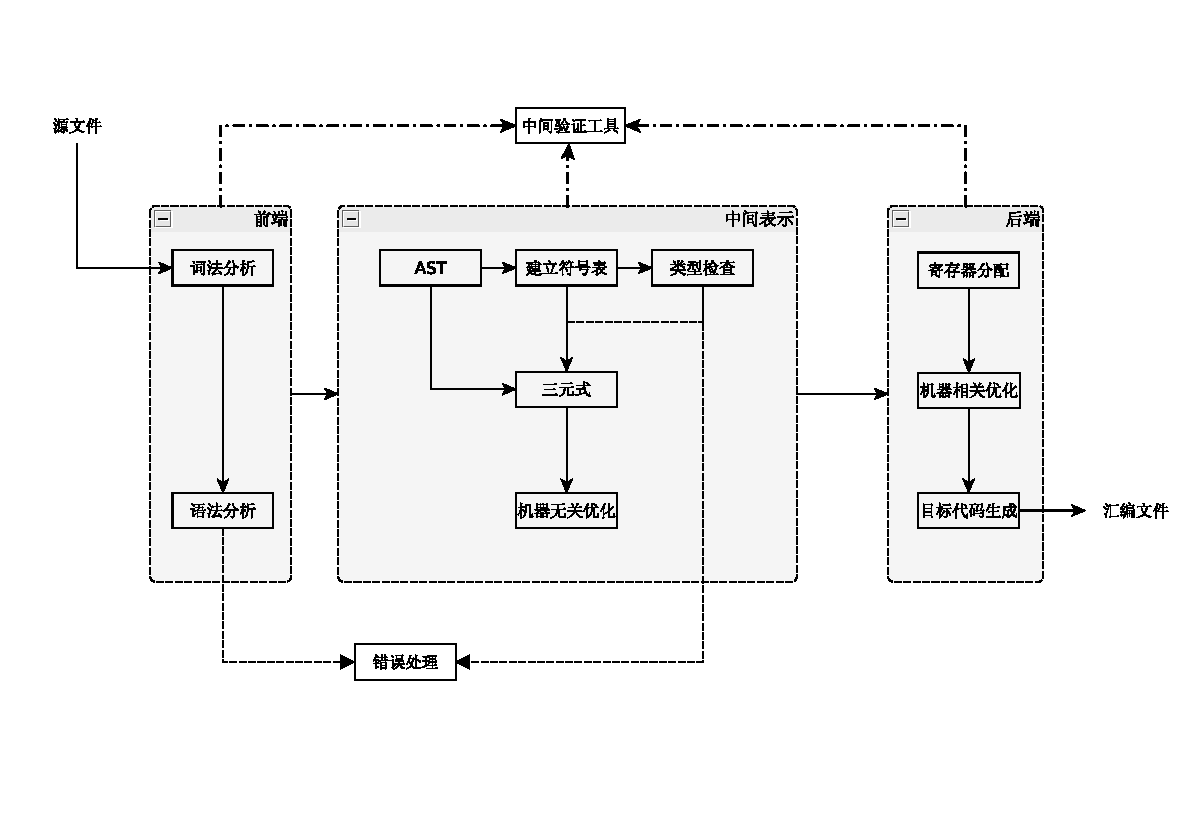
\includegraphics[scale=0.7]{main_structure.eps}
\end{center}
总体上看,MiniC由三大模块构成:
\begin{enumerate}
\item 前端:接收输入文件,结合文法,负责语法、词法分析;将源文件的结构和内容信息提取到抽象语法树(AST)上
\item 中间表示:共有两层:AST和三元式;语义分析在AST上完成后,将AST变换为三元式;机器无关优化在三元式表示上进行。
\item 后端:目标机器代码(汇编代码)生成;结合目标机器二进制规范和ISA,生成目标代码;机器相关优化在目标代码上进行。
\end{enumerate}
与此同时,还有错误处理模块,用于在源文件有误时产生出错提示;中间验证工具集,用于检查工程进展的每一个步骤的正确性。

在下面的章节中,我们将一一介绍以上模块。并且还将在最后一章展示MiniC编译器是如何与体系实习的模拟器项目配合,进行一系列编译-体系相关的实验。

\section*{致谢}
\begin{itemize}
\item 感谢刘先华老师对我们小组的指导。他总能及时、耐心地解答我们的问题,与此同时又鼓励我们积极思考和大胆尝试,使我们从这个实习项目中收获了知识和快乐。

\item 感谢刘锋老师在工程进展和规划、模拟器-编译器结合方面提供的帮助。

\item 感谢与我们一同选择MiniC项目的另外两个小组的成员,你们的帮助和启发使我们受益匪浅。

\item 当然,最需要感谢的是这个项目本身:我们通过它同时体验了CPU设计人员、模拟器设计人员、甚至是(一部分)操作系统设计人员在设计一个大型的、可靠的系统时所面临的挑战,以及克服这些挑战后所获得的成就感。
\end{itemize}

下面,我们将从头开始,介绍\textsc{Unicore-MiniC}编译器。

